% Created 2021-02-22 Mon 13:06
% Intended LaTeX compiler: pdflatex
\documentclass[english]{article}
\usepackage[T1, T2A]{fontenc}
\usepackage[lutf8]{luainputenc}
\usepackage[english, russian]{babel}
\usepackage{minted}
\usepackage{graphicx}
\usepackage{longtable}
\usepackage{hyperref}
\usepackage{xcolor}
\usepackage{natbib}
\usepackage{amssymb}
\usepackage{amsmath}
\usepackage{caption}
\usepackage{mathtools}
\usepackage{amsthm}
\usepackage{tikz}
\usepackage{grffile}
\usepackage{extarrows}
\usepackage{wrapfig}
\usepackage{rotating}
\usepackage{placeins}
\usepackage[normalem]{ulem}
\usepackage{amsmath}
\usepackage{textcomp}
\usepackage{capt-of}

\usepackage{geometry}
\geometry{a4paper,left=2.5cm,top=2cm,right=2.5cm,bottom=2cm,marginparsep=7pt, marginparwidth=.6in}

 \usepackage{hyperref}
 \hypersetup{
     colorlinks=true,
     linkcolor=blue,
     filecolor=orange,
     citecolor=black,      
     urlcolor=cyan,
     }

\usetikzlibrary{decorations.markings}
\usetikzlibrary{cd}
\usetikzlibrary{patterns}

\newcommand\addtag{\refstepcounter{equation}\tag{\theequation}}
\newcommand{\eqrefoffset}[1]{\addtocounter{equation}{-#1}(\arabic{equation}\addtocounter{equation}{#1})}


\newcommand{\R}{\mathbb{R}}
\renewcommand{\C}{\mathbb{C}}
\newcommand{\N}{\mathbb{N}}
\newcommand{\rank}{\text{rank}}
\newcommand{\const}{\text{const}}
\newcommand{\grad}{\text{grad}}

\theoremstyle{plain}
\newtheorem{axiom}{Аксиома}
\newtheorem{lemma}{Лемма}
\newtheorem{manuallemmainner}{Лемма}
\newenvironment{manuallemma}[1]{%
  \renewcommand\themanuallemmainner{#1}%
  \manuallemmainner
}{\endmanuallemmainner}

\theoremstyle{remark}
\newtheorem*{remark}{Примечание}
\newtheorem*{solution}{Решение}
\newtheorem{corollary}{Следствие}[theorem]
\newtheorem*{examp}{Пример}
\newtheorem*{observation}{Наблюдение}

\theoremstyle{definition}
\newtheorem{task}{Задача}
\newtheorem{theorem}{Теорема}[section]
\newtheorem*{definition}{Определение}
\newtheorem*{symb}{Обозначение}
\newtheorem{manualtheoreminner}{Теорема}
\newenvironment{manualtheorem}[1]{%
  \renewcommand\themanualtheoreminner{#1}%
  \manualtheoreminner
}{\endmanualtheoreminner}
\captionsetup{justification=centering,margin=2cm}
\newenvironment{colored}[1]{\color{#1}}{}

\tikzset{->-/.style={decoration={
  markings,
  mark=at position .5 with {\arrow{>}}},postaction={decorate}}}
\makeatletter
\newcommand*{\relrelbarsep}{.386ex}
\newcommand*{\relrelbar}{%
  \mathrel{%
    \mathpalette\@relrelbar\relrelbarsep
  }%
}
\newcommand*{\@relrelbar}[2]{%
  \raise#2\hbox to 0pt{$\m@th#1\relbar$\hss}%
  \lower#2\hbox{$\m@th#1\relbar$}%
}
\providecommand*{\rightrightarrowsfill@}{%
  \arrowfill@\relrelbar\relrelbar\rightrightarrows
}
\providecommand*{\leftleftarrowsfill@}{%
  \arrowfill@\leftleftarrows\relrelbar\relrelbar
}
\providecommand*{\xrightrightarrows}[2][]{%
  \ext@arrow 0359\rightrightarrowsfill@{#1}{#2}%
}
\providecommand*{\xleftleftarrows}[2][]{%
  \ext@arrow 3095\leftleftarrowsfill@{#1}{#2}%
}
\makeatother
\author{Ilya Yaroshevskiy}
\date{\today}
\title{Лекция 3}
\hypersetup{
 pdfauthor={Ilya Yaroshevskiy},
 pdftitle={Лекция 3},
 pdfkeywords={},
 pdfsubject={},
 pdfcreator={Emacs 28.0.50 (Org mode )}, 
 pdflang={English}}
\begin{document}

\maketitle
\tableofcontents

\newcommand{\X}{\mathcal{X}}
\newcommand{\A}{\mathfrak{A}}

\section{Интеграл}
\label{sec:orge2e6c11}
\begin{enumerate}
\item \(f \ge 0\), ступенчатые \\
\(f = \sum_\text{кон.} \alpha_k \chi_{E_k}\), \(E_k\) --- измеримое \\
\(\int_X f = \sum \alpha_k \mu E_k\)
\item \label{int_3_2} \(f \ge 0\), измеримая \\
\(\int_X f d\mu = \sup_{\substack{0 \le g \le g \\ f\text{ --- ступ.}}} \int_X g d\mu\)
\item \label{int_3_3} \(f\) --- измерима, \(f^+, f^- \ge 0\) --- измеримые \\
Пусть \(\int_X f^+\) или \(\int_X f^-\) --- конечные \\
Тогда \(\int_X f = \int_X f^+ - \int_X f^-\)
\begin{definition}
Если \(\int_x f^+,\ \int_X f^-\) --- оба конечные, то \(f\) назывется \textbf{суммируемой}
\end{definition}
\begin{remark}
\(f\) --- измеримая, \(\ge 0\), интеграл \ref{int_3_3} = интеграл \ref{int_3_2}
\end{remark}
\item \begin{definition}
\(E \subset X\) --- измкримое, \(f\) --- измерима на \(X\) \\
\(\int_E f d\mu = \int_X f\cdot\chi_E\)
\end{definition}
\end{enumerate}

\begin{remark}
\(f = \sum \alpha_k \chi_{E_k}\ \int_E f = \sum \alpha_k \mu(E_k \cap E)\)
\end{remark}
\begin{remark}
\(\int_E f d\mu = \sup \{fg:\ 0 \le g \le f\text{ на } E, g\text{ --- ступенчатые}\}\), можно считать что \(g\) ---
тождественный 0 вне множества \(E\)
\end{remark}
\begin{remark}
\(\int_E f\) не зависит от значений \(f\) вне \(E\)
\end{remark}
\begin{remark}
\((X, \A, \mu)\) \(E\subset X\) --- измеримое, \(g, f\) --- измеримые. Свойства:
\begin{enumerate}
\item \label{prop_3_1} Монотонность \(f \le g\) \(\int_E f \le \int_E g\)
\begin{proof}
\-
\begin{center}
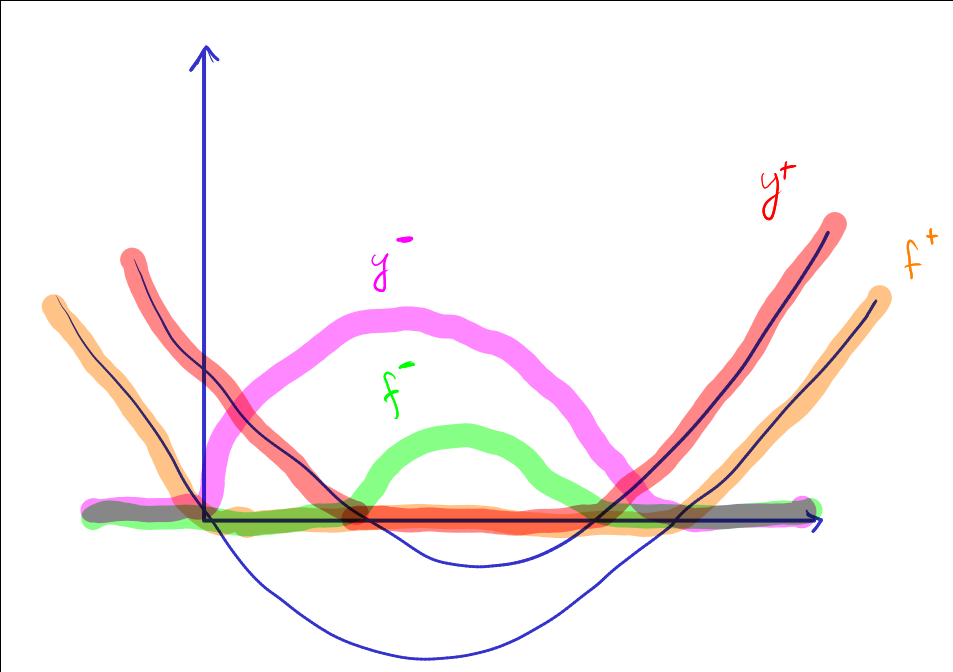
\includegraphics[scale=0.3]{3_1.png}
\end{center}
\begin{enumerate}
\item \(f, g \ge 0\) --- очевидно
\item \(f, g\) --- произвольные \\
\(f^+ \le g^+\ f^- \le g^-\) \\
\(\int_E f^+ \le \int_E g^+\ \int_E f^- \le \int_E g^- \Rightarrow \text{OK}\)
\end{enumerate}
\end{proof}
\item \(\int_E Ad\mu = \mu E\ \int_E 0 d\mu = 0\)
\item \label{prop_3_3} \(\mu E = 0\ \int_E f= 0\)
\begin{proof}
\begin{enumerate}
\item \(f\) --- ступенчатая
\item \(f \ge 0\) --- измеримая
\end{enumerate}
\end{proof}

\emph{Змечание}: \\
\(f\) --- измеримая. Тогда \(f\) --- суммируемая \(\Leftrightarrow\) \(\int |f| < + \infty\) \\
\begin{description}
\item[{\((\Leftarrow)\)}] следует из cвойства \ref{prop_3_1}. \(f^+, f^- \le |f|\)
\item[{\((\Rightarrow)\label{remark_3_1_proof}\)}] позже
\end{description}
\item \label{prop_3_4} \(\int_E(-f) = -\int_E f,\ \forall c \in \R\ \int_E c f = c\int_E f\) \\
\begin{enumerate}
\item \((-f)^+ = f^-\ (-f)^- = f^+\)
\item можно считать \(c > 0\) для \(f \ge 0\) --- тривиально
\end{enumerate}
\item \(\exists \int_E f d\mu\) \\
Тогда \(|\int_E f d\mu| \le \int_E |f| d\mu\)
\begin{proof}
\(-|f| \le f \le |f|\). По свойствам \ref{prop_3_3} и \ref{prop_3_4}
\end{proof}
\item \(\mu E \le +\infty,\ a\le f\le b\) \\
Тогда \(a\mu E \le \int_E f \le b \mu E\)
\(\color{gray} a\chi_E \le f \le b\chi_E\)
\begin{corollary}
\(f\) --- измерима на \(E\), \(f\) --- ограничена на \(E\), \(\mu E < + \infty\) \\
Тогда \(f\) --- суммируемая на \(E\)
\end{corollary}
\item \(f\) --- суммируемая на \(E\). Тогда \(f\) --- почти везде конечная
\begin{proof}
\-
\begin{enumerate}
\item \(f \ge 0\ f = + \infty\) на \(A \subset E\) \(\forall n \in \N\ \int_E f \ge n\mu A\)
\item \(f = f^+ - f^-\)
\end{enumerate}
\end{proof}
\end{enumerate}
\end{remark}
\begin{lemma}
\label{lemma_3_1}
\[ A = \bigsqcup_{i - 1}^{ + \infty} A_i \]
--- измеримые, \(g\) --- ступенчатая, \(g \ge 0\) \\
\uline{Тогда} \[ \int_A g d\mu = \sum_{i = 1}^{ + \infty}\int_{A_i}g d\mu \]
\end{lemma}
\begin{proof}
\(\int_A g d\mu = \sum_\text{кон.} \alpha_k \mu(E_k \cap A) = \sum_k\sum_i \underbrace{\alpha_k\mu(E_k \cap A_i)}_{\ge 0} = \sum_i \sum_k \dots = \sum_i\int_{A_i} gd\mu\)
\end{proof}
\begin{theorem}
\(A = \bigsqcup A_i\) --- измеримые, \(f: X \to \overline{\R}\) --- измеримая на \(A\), \(f \ge 0\) \\
\uline{Тогда} \(\int_A fd\mu = \sum_{i = 1}^{ + \infty} \int_{A_i} f d\mu\)
\end{theorem}
\begin{proof}
\-
\begin{description}
\item[{\((\le)\)}] ступенчатая \(g:\ 0 \le g \le f\ \int_a g = \sum\int_{A_i} g d\mu \le \sum \int_{A_i} f\) --- по \hyperref[lemma_3_1]{Лемме}
\item[{\((\ge)\)}] \begin{enumerate}
\item \(A = A_1 \cup A_2\) \\
\(0 \le g_1 \le f\chi_{A_1}\ 0 \le g_2 \le f\chi_A_2}\) \\
\[ g_1 = \sum \alpha_k \chi_{E_k}\ g_2 = \sum \beta_k \chi_{E_k} \]
\begin{center}
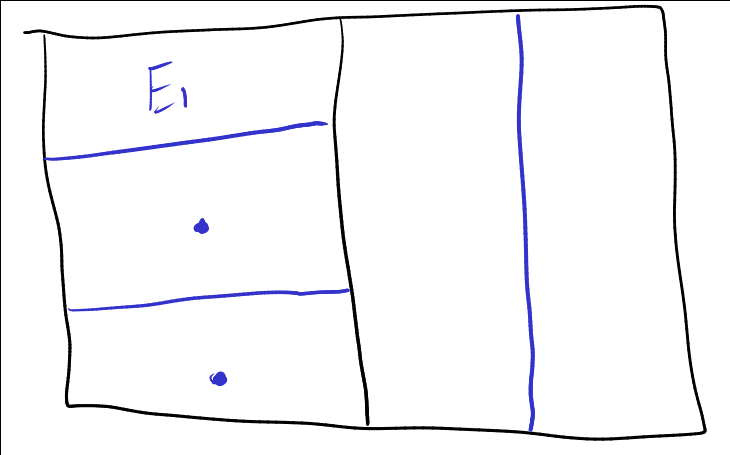
\includegraphics[scale=0.3]{3_2.png}
\end{center}
Считаем что \(E_k\) -- совместное разбиение
\[ 0 \le g_1 + g_2 \le f \chi_A \]
\[ \int_{A_1} g_1 + \int_{A_2} g_2 =  \int_A g_1 + g_2 \le \int_A f \]
Перейдем к супремуму
\[ \int_{A_1} f + \int_{A_2} g_2 \le \int_A f \]
\[ \int_{A_1} f + \int_{A_2} f \le \int_A f \]
\item \(\forall n \in \N\) --- индукция по \(n\)
\item \[ A = \bigsqcup_{i = 1}^n A_i \sqcup B_n \], где \[ B_n = \bigsqcup_{i > n} A_i \]
\[ \int_A f = \sum_{i = 1}^n \int_{A_i} f + \int_{B_n} f \ge \sum_{i = 1}^n \int_{A_i} f \]
\end{enumerate}
\end{description}
\end{proof}
\begin{corollary}
\begin{itemize}
\item \(f \ge 0\) --- измеримая
\item \(\nu: \A \to \overline{\R}_+\)
\item \(\nu E := \int_E fd\mu\)
\end{itemize}
\uline{Тогда} \(\nu\) --- мера
\end{corollary}
\begin{corollary}[аддитивности интеграла]
\(f\) --- суммируема на \(A = \bigsqcup A_i\) --- измеримые \\
\uline{Тогда} \[ \int_A f = \sum \int_{A_i} f \]
\end{corollary}
\begin{proof}
\(f^+, f^- \dots\) \(\color{red}???\)
\end{proof}
\subsection{Предельный переход под щнаком интеграла}
\label{sec:orgdfeb008}
\(f_n \to f\). Можно ли утверждать \(\int_E f_n \to \int_E f\)?
\begin{examp}
\(f_n, f: \R \to \R\) \\
\(f_n = \frac{1}{n} \cdot \chi_{[0, n]}\ f\equiv 0\ f_n \to f\) (даже \(f_n \rightrightarrows f\) на \(\R\)) \\
\[ \int_\R f_n = \frac{1}{n}\lambda[0, n] = 1\not \xrightarrow[n \to + \infty]{} 0 = \int_\R f \]
\end{examp}
\begin{theorem}[Леви]
\((X, \A, \mu)\), \(f_n\) --- измеримая \\
\(\forall n\ 0 \le f_n \le f_{n + 1}\)  почти везде \(f(x) := \lim_{n\to + \infty} f_n(x)\) почти везде \\
\uline{Тогда} \(\lim_{n \to + \infty}\int_X f_n d \mu = \int_x fd\mu\)
\end{theorem}
\begin{remark}
\(f\) --- задана всюду, кроме множества меры \(0\). Считаем, что \(f = 0\) на \(e\) \\
\uline{Тогда} \(f\) --- измерима на \(X\).
\end{remark}
\begin{proof}
\-
\begin{description}
\item[{\((\le)\)}] очевидно. \(f_n \le f\) почти везде \(\int f_n \le \int f\)
\[ \int_X f_n = \int_{X\setminus e}f_n + \int_e f_n = \int_{X\setminus e} f_n \le \int_{X \setminus e} f \le \int_X f \]
\item[{\((\ge)\)}] Достаточно: \(\forall g\) --- ступенчатая \(0 \le g \le f\)
\[ \lim \int_X f_n \ge \int_X g \]
Достаточно: \(\forall c \in (0, 1)\)
\[ \lim \int_X f_n \ge c \int_X g \]
\[ E_n := X(f_n \le c g) \dots \subset E_n \subset E_{n + 1} \subset \dots \]
\(\bigcup E = X\) т.к. \(c < 1\)
\[ \int_x f_n \ge \int_{E_n} f_n \ge c \int_{E_n} g \]
Тогда \(\lim \int_X f_n \ge c \lim \int_{E_n} g = c\int_X g\) \\
Последнее равентсво справедливо в силу непрерывности мнизу меры \(\nu: E \mapsto \int_E g\)
\end{description}
\end{proof}

\begin{theorem}
\(f, g \ge 0\) измерима на \(E\) \\
\uline{Тогда} \[ \int_E f + g = \int_E f + \int_E g \]
\end{theorem}
\begin{proof}
\-
\begin{enumerate}
\item \(f, g\) --- ступенчатые \\
\[ f = \sum \alpha_k\chi_{E_k},\ g = \sum \beta_k\chi_{E_k} \]
\[ \int_E f + g = \sum (\alpha_k + \beta_k)\mu(E_k \cap E) = \sum \alpha_k \mu(E_k \cap E) + \sum \beta_l \mu(E_k \cap E) = \int_E f + \int_E g \]
\item \(f \ge 0\) --- измерима \(\Rightarrow\) \(\exists\) стпенчатая \(f_n:\ 0 \le f_n \le f_{n + 1} \le \dots \ \lim f_n = f\) \\
\(g \ge 0\) --- измерима \(\Rightarrow\) \(\exists\) стпенчатая \(g_n:\ 0 \le g_n \le g_{n + 1} \le \dots \ \lim g_n = g\) \\
\(f_n + g_n \to f + g\ \int_E f_n + g_n \to \int_E f + g\) \\
\(\int_E f_n + g_n = \int_E f_n + \int_E g_n \to \int_E f + \int_E g = \int_E f+g\)
\end{enumerate}
\end{proof}
\begin{corollary}
\(f, g\) --- суммируемы на \(E\) \\
\uline{Тогда} \(f+g\) --- суммируема и \(\int_E f + g = \int_E f + \int_E g\)
\end{corollary}
\begin{remark}
Свойство \(\ref{remark_3_1_proof}\) доказано
\end{remark}
\begin{proof}
Суммируемость \(|f+g|\le |f| + |g|\) \\
\(h = f + g\). Тогда:
\[ h^+ - h^- = f^+ - f^- + g^+ - g^- \Leftrightarrow h^+ + f^- + g^- = h^- + f^+ + g^+ \]
\[ \Rightarrow \int_E h^+ + \int_E f^- + \int_E g^- = \int_E h^- + \int_E f^+ + \int_E g^+ \]
\[ \int_E h^+ - \int_E h^- = \int_E f^+ - \int_E f^- + \int_E g^+ - \int_E g^- \]
\[ \int_E h = \int_E f + \int_E g \]
\end{proof}
\begin{definition}
\(\mathcal{L}(X) =\) множество функций суммируемых на X
\end{definition}
\begin{corollary}
\(\mathcal{L}(X)\) --- линейное пространство, а отображение \(f \mapsto \int_X f\) --- это линейный функционал на \(\mathcal{L}(X)\)
, т.е. \(\forall f_1, \dots, f_n \in \mathcal{L}(X)\ \forall \alpha_1, \dots, \alpha_k \in \R\)
\[ \sum_{k = 1}^n \alpha_k f_k \in \mathcal{L}(X);\ \int_X\sum\alpha_k f_k = \sum_{k = 1}^n\alpha_k\int_X f_k\]
\end{corollary}
\begin{theorem}[об интегрировании положительных рядов]
\((X, \A, \mu)\ E \in \A\ \underset{\text{изм.}}{u_n}: X \to \overline{\R}\ u_n \ge 0\) почти везде \\
\uline{Тогда} \[ \int_E(\sum_{n = 1}^{ + \infty} u_n(x))d\mu(x) = \sum_{n = 1}^{ + \infty} \int_E u_n d\mu \]
\end{theorem}
\begin{proof}
по т. Леви: \(S_n := \sum_{k = 1}^n u_k\ 0 \le S_n \le S_{n + 1} \le \dots\ S_n \to S\) --- сумма ряда \(\sum u_n\) \\
Тогда \(\int_E S_n \to \int_E S\), \(\int_E S_n = \sum_{k = 1}^n \int_E u_k \to \int_E S\)
\end{proof}
\begin{corollary}
\(u_n\) --- измеримые \(\sum_{n = 1}^{ + \infty} \int_E |u_n| < + \infty\) \\
\uline{Тогда} ряд \(\sum u_n(x)\) --- абсолютно сходится при почти всех \(x\)
\end{corollary}
\begin{proof}
\(S(x) := \sum |u_n(x)| \ge 0\) --- измеримая
\[ \int_E S(x) = \sum \int_E |u_n| < + \infty \]
\(\Rightarrow\) \(S\) --- сумиируема \(\Rightarrow\) \(S\) почти везде конечена
\end{proof}
\begin{examp}
\(x_n \in \R\) --- произведение последовательности; \(\sum a_n\) --- абсолютно сходится \\
\uline{Тогда} \(\sum \frac{a_n}{\sqrt{|x - x_n|}}\) --- абсолютно сходится при почти всех \(x\)
\end{examp}
\begin{proof}
Достаточно проверить абсолютную сходимость на \([-N, N]\) почти везде
\begin{center}
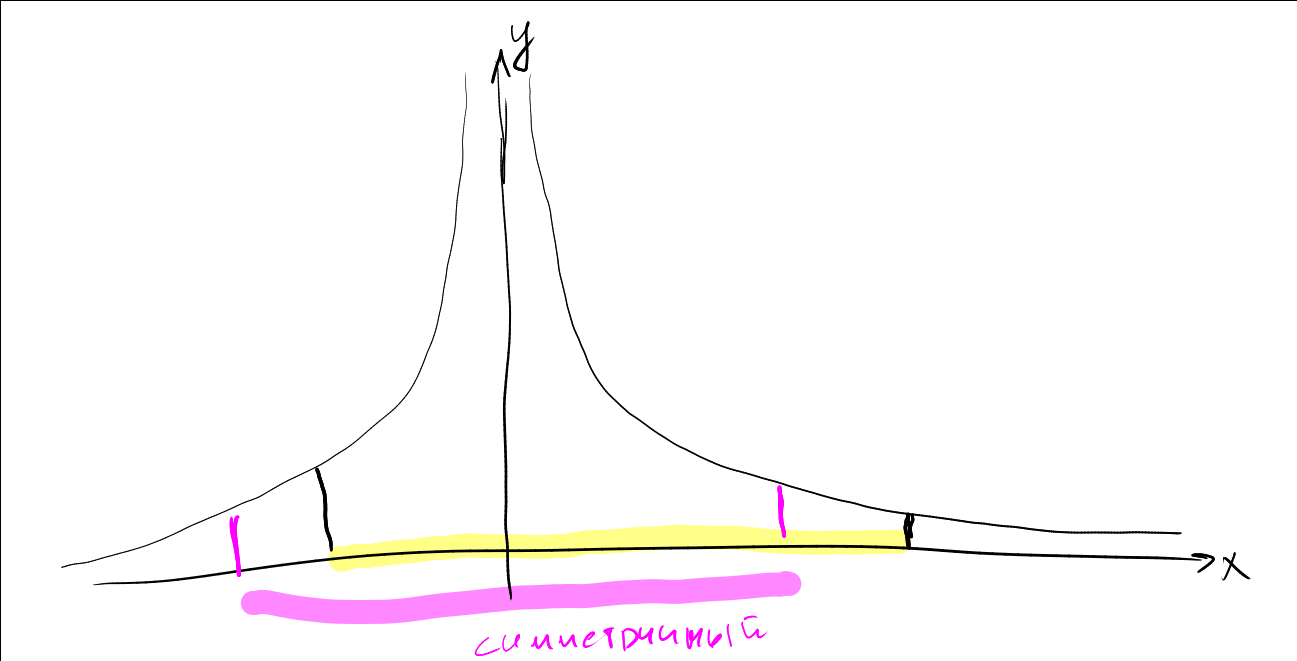
\includegraphics[scale=0.3]{3_3.png}
\end{center}
\[ \int_{[-N , N]} \frac{|a_n|}{\sqrt{|x - x_n|}} = \int_{-N}^N \frac{|a_n|}{\sqrt{|x - x_n|}} dx = |a_n| \int_{-N - x_n}^{N - x_n} \frac{dx}{\sqrt{|x|}} \le \]
\[ \le |a_n| \int_{-N}^N \frac{dx}{\sqrt{|x|}} = 4\sqrt{N}\cdot|a_n| \]
\[ \sum_n \int_{[-N, N]}\frac{|a_n|}{\sqrt{|x - x_n|}} \le 4 \int_N \sum |a_n| < + \infty \]
\end{proof}
\end{document}
